\chapter{Results and Discussion}\label{chap:7}
The results presented here concern the three-body effective potential curves obtained by solving \Cref{adiabatic} within the strict adiabatic treatment, see \Cref{sec:Effective_3B}. Signatures of the Efimov effect can be revealed in the structure of these adiabatic hyperspherical potentials, with the Efimov channel corresponding to the one emergent attractive potential converging to \eqref{eq:efimov_channel} in the region $r_0 \ll \rho \ll
\abs{a}$.

The adiabatic potential curves were obtained by numerically solving \Cref{adiabatic} in  two-dimensional hyperangular space at fixed hyperradii using the method outlined in \Cref{chapter:5}. The two-body scattering model described in \Cref{chapter:scattering_model} was used with the interaction range fixed at $r_0=55$ a.u. and with masses corresponding to the bosonic rubidium isotope $m = m( \prescript{87}{}{\mathrm{Rb}})$. 

We expect the potential curves to converge towards \eqref{eq:efimov_channel} for $\abs{a} \rightarrow \infty$. This behaviour is more easily recognized if the potentials are multiplied by $2 \mu \rho^2$ and plotted as 

\begin{equation}\label{eq:lambda}
\xi(\rho) = 2 \mu \rho^2 W_{\nu}(\rho) + \frac{1}{4},
\end{equation}
since these curves should approach the universal value $-s_0^2 (\simeq -1.0125$ for $J=0^+$ states) for the lowest effective potential. This scenario is restricted to the range $r_0 \ll \rho \ll \abs{a}$ and we only expect to find a potential $\xi(\rho)$ that is infinitely extended towards this universal value in the resonant regime when the magnitude of the scattering length is infinite. In this regime, the solution $\xi_{\infty}(\rho/\abs{a}) = -s_0^2$ gives rise to an effective attractive potential, which is proportional to $\rho^{-2}$. This effective attractive potential is substituted into the hyperradial equation \eqref{fullhamiltonian}, where it in turn results in an infinite number of bound trimer states.

We start by exploring Efimov's original scenario for two effective potentials calculated with two-body interactions very close to the resonant regime $a \approx \pm \infty$. The values of the potential depths $d$ were tuned near the pole labelled $\mathrm{I}$ in \Cref{fig:res_1}, so that the two-body potential was just short of, or could just barely, support a single two-body bound state. To confirm the validity of the code the convergence of the adiabatic eigenvalues was tested over a broad range of hyperradii $\rho$ using an increasing number of B-splines in each hypersperical dimension. 

In \Cref{table:Res_2} we present a systematic analysis of the numerical potential values $\xi(\rho)$ for the two cases where the scattering length was tuned to $a_1 \rightarrow -\infty$ and $a_2 \rightarrow \infty$. The adiabatic eigenvalues were calculated at ten different hyperradial points using $40$, $60$, $80$ and $100$ B-splines in each coordinate dimension. The convergence of our numerical potentials for values of $\rho$ up to $\rho_{max} = 2 \times 10^4$ a.u. is indictated by the fact that the numerical values for the three-body effective potential energies are virtually unaffected by increasing the number of B-splines past $N_{\theta}=80$. We also observe numerical convergence towards the universal constant $-s_0^2$ for $\rho \approx 1.5 \times 10^4$ a.u. 

\begin{table}[h!]
	\centering
	\footnotesize
	\begin{adjustwidth}{-0.1cm}{}
		\tabcolsep=0.10cm
		\begin{tabular}{||c c c c c c c||} 
			\hline
			$a$ (a.u.) & $N_{\theta}$ & $\xi(\rho = 10 $ a.u.) & $\xi(100 $ a.u.) & $\xi(1000 $ a.u.) & $\xi(5000 $ a.u.) & $\xi(10000 $ a.u.)  \Tstrut\Bstrut \\ [0.7ex]
			\hline\hline  \Tstrut\Bstrut 
			$a_1$   & 40  & 3.77527814 & $-$2.60368386 & $-$1.13917612 & $-$1.03381510& $-$1.01875934 \\
			$a_1$   & 60  & 3.77527815 & $-$2.60368387 & $-$1.13917795 & $-$1.03402416& $-$1.01912287\\
			$a_1$   & 80  & 3.77527829 & $-$2.60368372 & $-$1.13917758 & $-$1.03402814 & $-$1.01913548 \\
			$a_1$   & 100  & 3.77530687 & $-$2.60367682 & $-$1.13917744 & $-$1.03405123 & $-$1.01907622 \\ [0.5ex]
			\hline \Tstrut\Bstrut 
			$a_2$   & 40  & 3.77526187 & $-$2.60416379 & $-$1.14059416 & $-$1.04035561 & $-$1.03170806 \\
			$a_2$   & 60  & 3.77526187 & $-$2.60416379 & $-$1.14058505 & $-$1.04056429 & $-$1.03207319 \\
			$a_2$   & 80  & 3.77526202 & $-$2.60416364 & $-$1.14059531 & $-$1.04056828 & $-$1.03208588 \\
			$a_2$   & 100  & 3.77526910 & $-$2.60416170 & $-$1.14059544 & $-$1.04056460 & $-$1.03224690 \\ [0.7ex] 
			\hline
			\hline
			$a$ (a.u.) & $N_{\theta}$ & $\xi(14900 $ a.u.) & $\xi(15000 $ a.u.) & $\xi(16000 $ a.u.) & $\xi(18000 $ a.u.) & $\xi(20000 $ a.u.)  \Tstrut\Bstrut \\ [0.7ex]
			\hline\hline  \Tstrut\Bstrut 
			$a_1$   & 40  & $-$1.01212794 & $-$1.01201907 & $-$1.01096344 & $-$1.00898721& $-$1.00713887 \\
			$a_1$   & 60  & $-$1.01250002& $-$1.01239205 & $-$1.01134995 & $-$1.00943386 & $-$1.00768456 \\
			$a_1$   & 80 & $-$1.01251258 & $-$1.01240463 & $-$1.01136253 & $-$1.00944703 & $-$1.00770029 \\
			$a_1$   & 100  & $-$1.01252039 & $-$1.01240591 & $-$1.01136323 & $-$1.00944484& $-$1.00769736 \\[0.5ex]
			\hline  \Tstrut\Bstrut 
			$a_2$   & 40 & $-$1.03136024 & $-$1.03137963 & $-$1.03160655 & $-$1.03219548 & $-$1.03291215 \\
			$a_2$   & 60 & $-$1.03173469 & $-$1.03175499 & $-$1.03199569 & $-$1.03264544 & $-$1.03346237 \\
			$a_2$   & 80  & $-$1.03174732 & $-$1.03176769 & $-$1.03200835 & $-$1.03265878 & $-$1.03347809 \\
			$a_2$   & 100 & $-$1.03174824 & $-$1.03176640 & $-$1.03200773 & $-$1.03265632 & $-$1.03347886 \\ [0.7ex] 
			\hline
		\end{tabular}
	\end{adjustwidth}
	\caption{Three-body effective potential energy values $\xi(\rho)$ at different hyperradii for $a_1 = -2702020$ a.u. and $a_1 = 1966590$ a.u. The potential for $a<0$ has converged, while the potential for $a>0$ tends to converge to the universal value $-s_0^2 \simeq -1.01251$ at hyperradii close to $\rho=15000$ a.u.}
	\label{table:Res_2}
\end{table} 

In \Cref{fig:infty} we show the results obtained over the full hyperradial range up to $2 \times 10^4$ a.u., where the numerically calculated three-body effective potentials $\xi(\rho)$ are plotted as functions of $\rho$. Note the logarithmic scale on the hyperradial axis. The curves can here be seen to converge towards the characteristic universal value $-s_0^2$ for $\rho \gg r_0$. 

\begin{figure}[h!]
	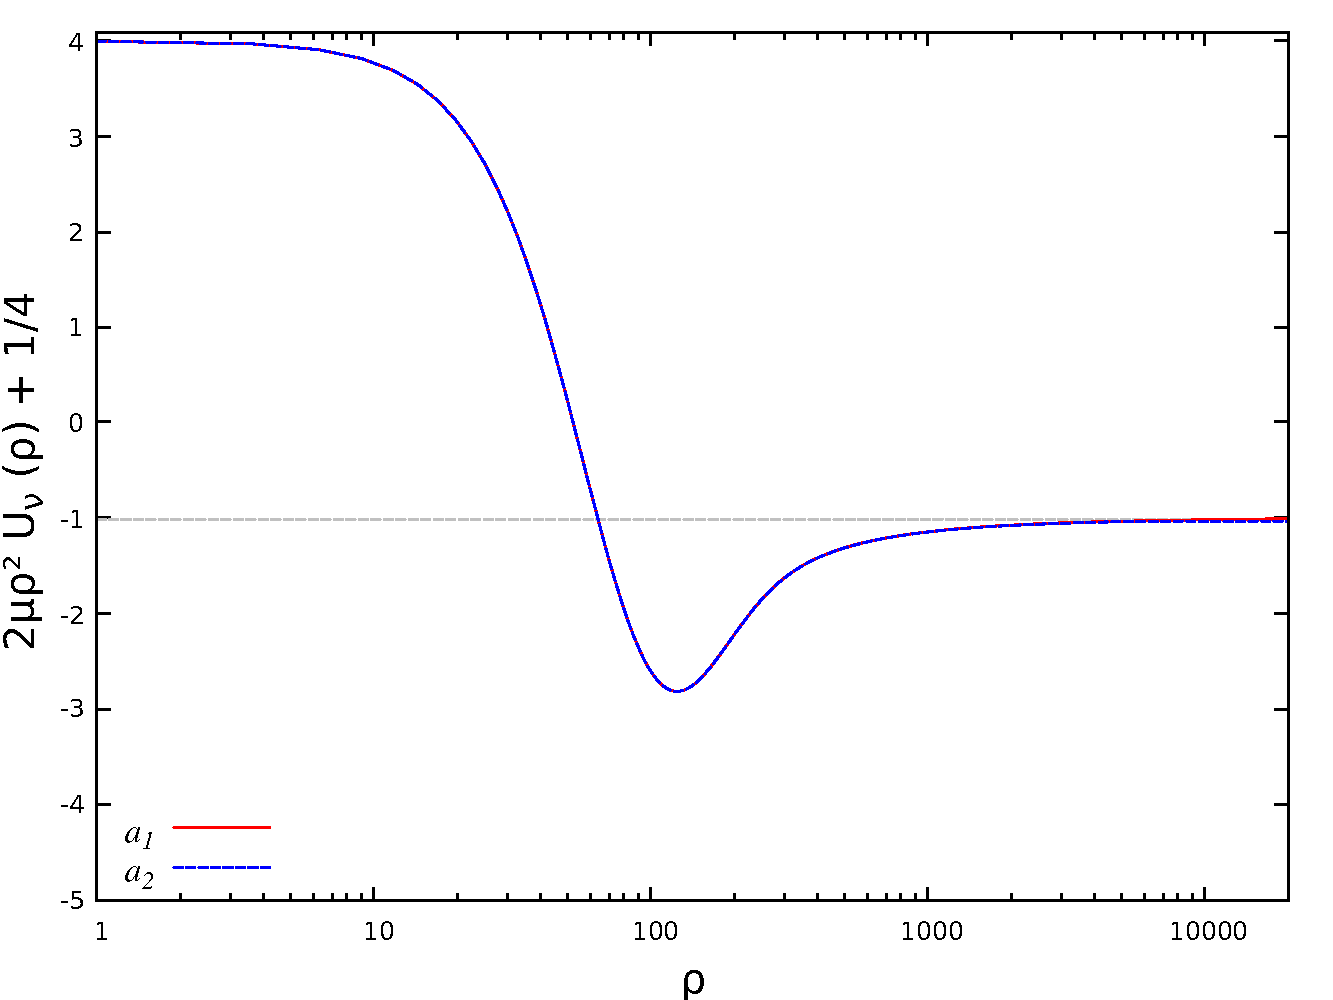
\includegraphics[width=\linewidth]{infty.pdf}
	\caption{The lowest three-body effective potential curves $\xi(\rho)$ are plotted as functions of $\rho$ for $a_1 = -2702020$ a.u. and $a_1 = 1966590$ a.u. over the full range of hyperradii for which the numerically calculated potentials converged.}
	\label{fig:infty}
\end{figure}

For all results presented in this chapter we were able to achieve convergence using a uniformly spaced mesh for hyperradii out to $\rho \approx 5 \times 10^3$ a.u. However, at larger hyperradii the two-body potential surface $V(\rho,\theta,\phi)$ changes much more rapidly near the coalescence points, i.e., at the hyperangular configurations $(\theta,\phi) = (\pi/2,\phi)$, $(\pi/2,\phi - 2\pi/3)$ and $(\pi/2,\phi - 2\pi/3)$. In \Cref{fig:surfaces} the two-body potential surfaces are plotted at two different hyperradii to illustrate how the size of the system changes the numerical complexity. To account for the increased numerical difficulties with increasing system size, the grid was more densly packed near the boundary $(\theta,\phi)=(\pi/2,\pi/3)$ for $\rho > 5 \times 10^3$ a.u. By doing this, we were able to achieve convergence out to $\rho \approx 2 \times 10^4$ a.u. and we can probably get convergence out to even larger $\rho$ by further improving the knot point distribution on the grid.

Next, we consider the near-resonant scenario for finite $a$. For short-ranged two-body potentials where the magnitude of the scattering length is large but finite we expect that the effective potentials $W_{\nu}(\rho)$ are to some extent affected by Efimov physics in the range $r_0 \ll \rho \ll \abs{a}$ and that the lowest effective potentials obtained with a larger magnitude of $a$ exhibit closer resemblence with the true Efimov potential given in \Cref{eq:lambda}. However, in the asymptotic limit $\rho \rightarrow \infty$, when $\rho \ll \abs{a}$ is not fulfilled, we anticipate that the behaviour of $W_{\nu}(\rho)$ depends on the sign of $a$, since it indicates whether or not the two-body interaction is strong enough to support a binary state and henceforth indicates the associated break-up channel. For $a>0$ the effective potentials $W_{\nu}(\rho)$ are expected to converge asymptotically to the energy of the weakly bound dimer \eqref{eq:weakdimer}. For $a<0$ we instead expect that the effective potentials $W_{\nu}(\rho)$ asymptotically approach \eqref{eq:continuumchannel}, i.e., the eigenvalues of the kinetic energy, which for the lowest potential $\xi(\rho)$ corresponds to $\lambda(\lambda + 4) + 4$ with $\lambda = 0$.

In \Cref{fig:res_5} the potential curves for $a>0$, asymptotically associated with the weakly bound dimer channel $\nu = 0$, are plotted as functions of the hyperradius $\rho$ for four different values of $a$. The results presented in this figure were obtained using values of $d$ that approached pole $\mathrm{I}$ from the right, thus supporting a single two-body bound state. The Efimov-like character of the three-body effective potentials is manifested by the flattening behaviour of the curves over an extended region in the intermediate range $r_0 \ll \rho \ll |a|$, which tend to converge towards the universal value $-s_0^2$ (indicated in the figure by the horizontal dashed line), as the magnitude of the scattering length is gradually increased. The asymptotic convergence of the effective potentials $W_{\nu}(\rho)$ to the channel of one weakly bound dimer and a free atom can in this figure be recognized by $\xi(\rho)$ displaying a parabolic dependence on $\rho$ in the asymptotic limit for each state. We highlight this behaviour for the two effective potentials obtained with the smallest values of $a$ in \Cref{fig:finite_conv} by including the two asymptotic forms $\xi_+ = 2\mu \rho^2 E_{2b} + 1/4$, calculated from the two-body energy $E_{2b}$ given in \Cref{eq:exact_2b}.   

\begin{figure}[htbp!]
	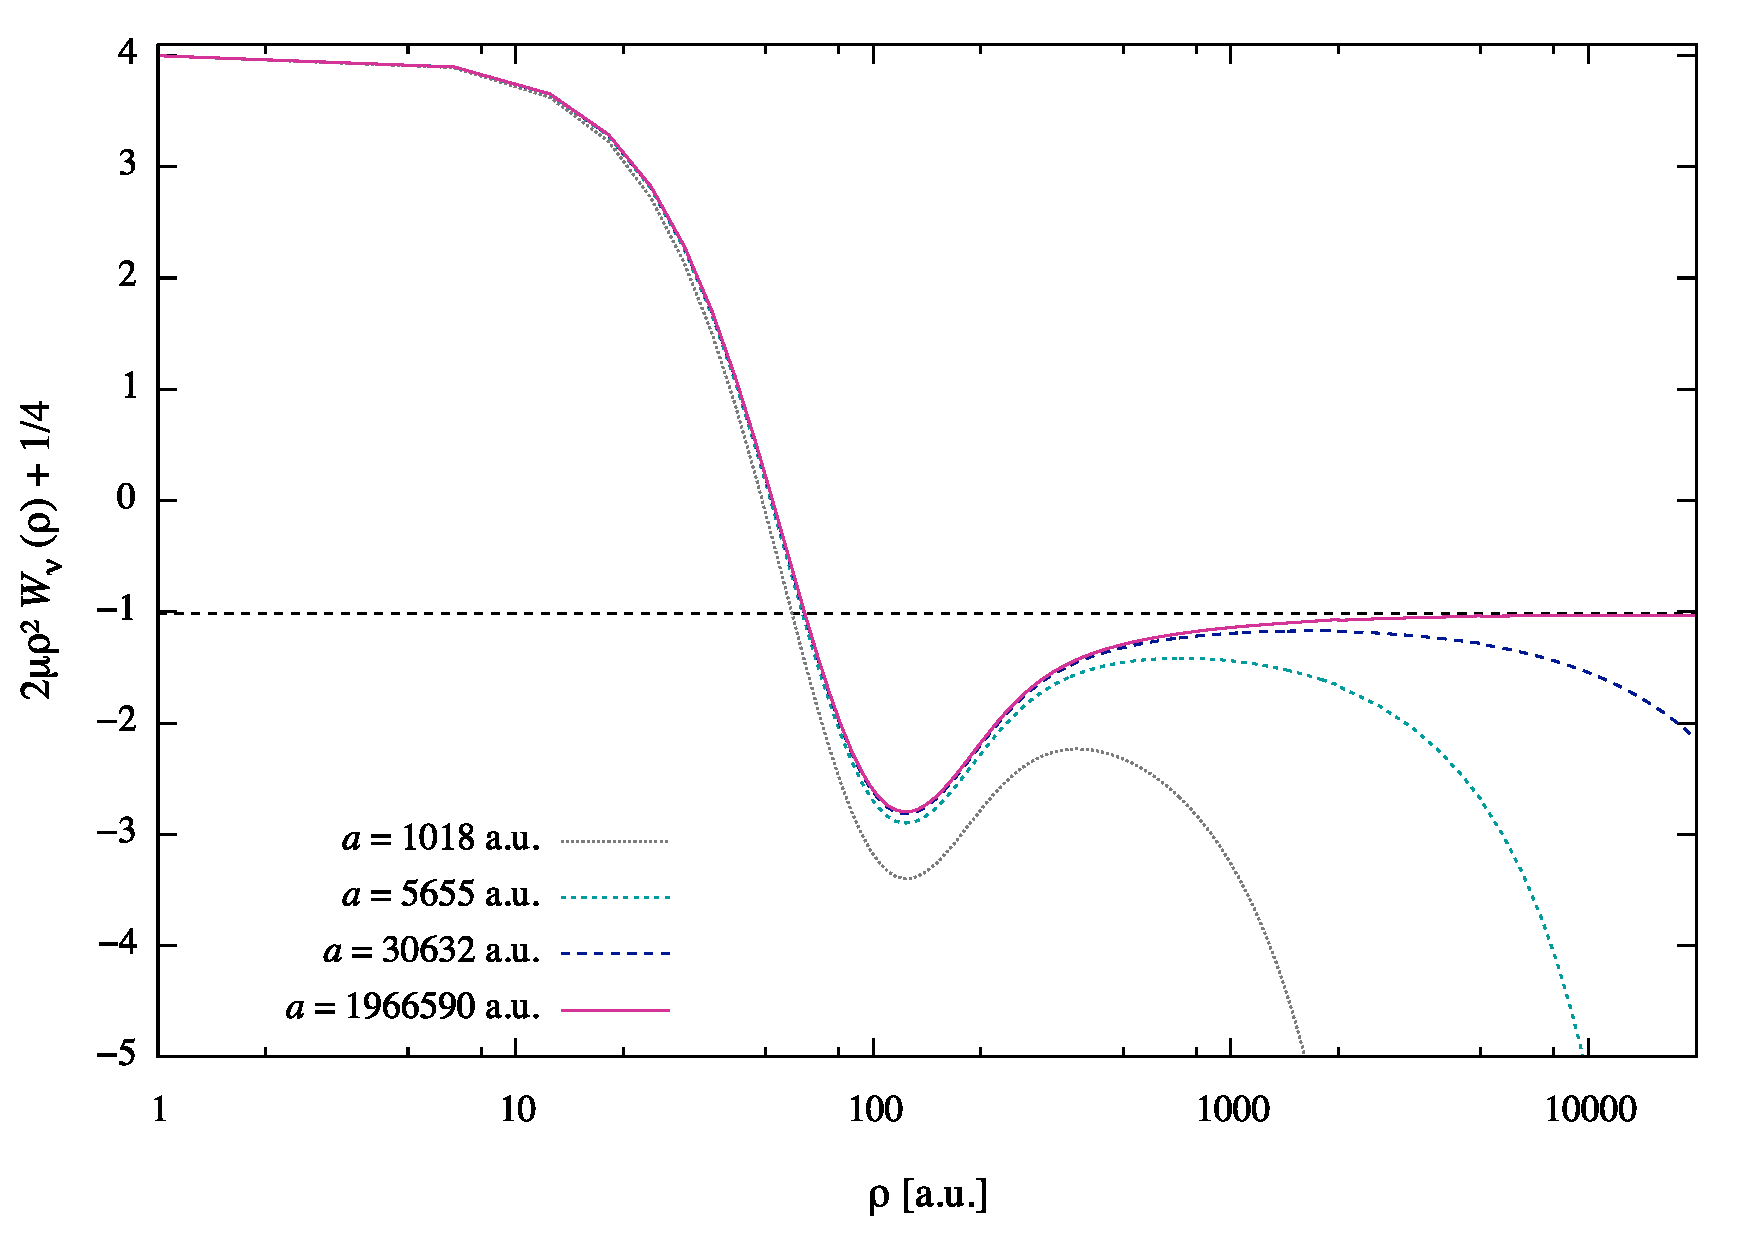
\includegraphics[width=\linewidth]{finite_positive_a.pdf}
	\caption{Three-body effective potentials for $a>0$. The horizontal dashed line is the universal value $-s_0^2$, which the Efimov potential takes on for $\rho\gg r_0$.}
	\label{fig:res_5}
\end{figure}

\begin{figure}[htbp!]
	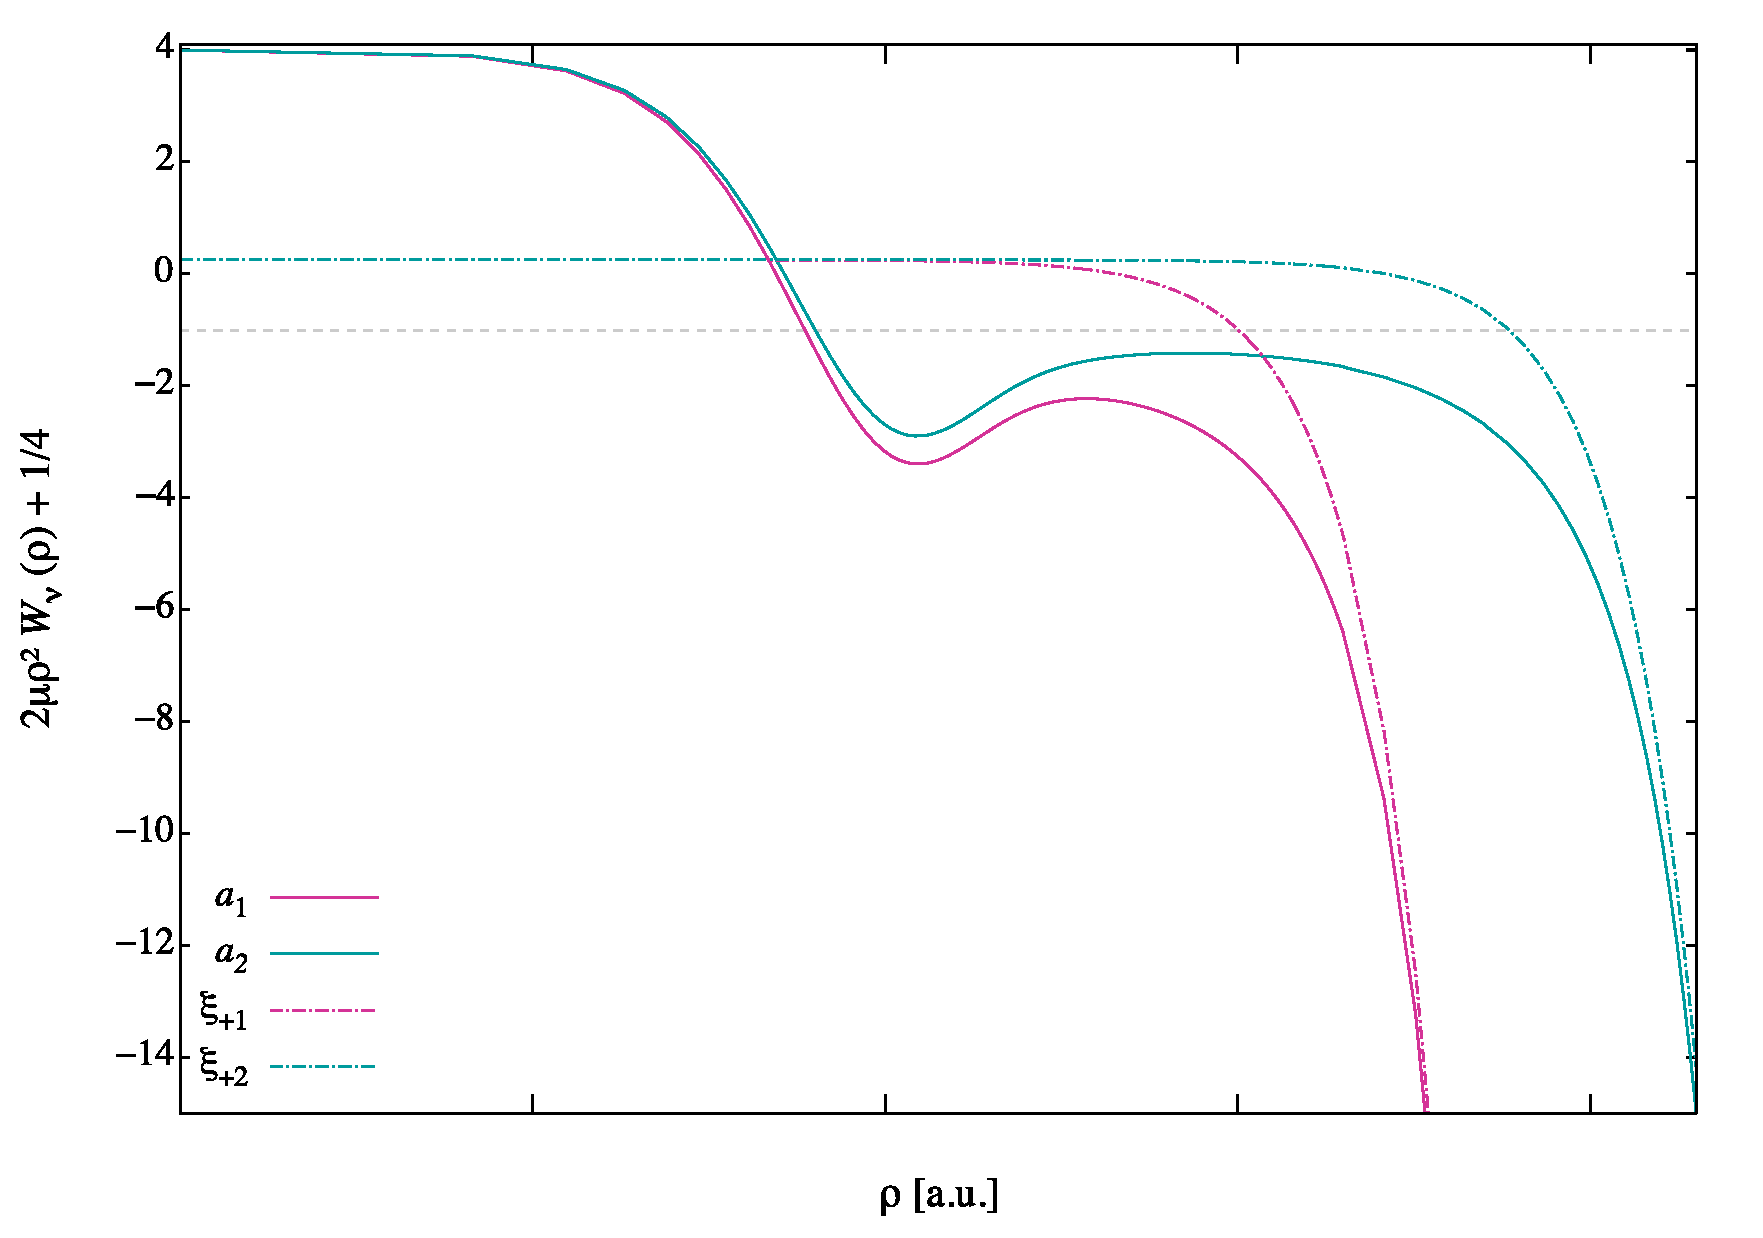
\includegraphics[width=\linewidth]{finite_conv.pdf}
	\caption{Three-body effective potentials for $a_1=1018$ a.u. and $a_2=5655$ a.u. are highlighted and shown together with their analytical asymptotic forms $\xi_{+1}$ and $\xi_{+2}$. The grey horizontal dashed line is the universal value $-s_0^2$.}
	\label{fig:finite_conv}
\end{figure}

In \Cref{fig:res_3} the potential curves for $a<0$, asymptotically associated with the lowest continuum channel, are plotted as functions of the hyperradius $\rho$ again for four different values of $a$. These three-body effective potentials also exhibit Efimov-like characteristics in the range $r_0 \ll \rho \ll |a|$, which can be discerned from the tendency of the potential curves to converge to $-s_0^2$ as the magnitude of $a$ increases, while they return to the kinetic energy in the asymptotic limit.

\begin{figure}[htbp!]
	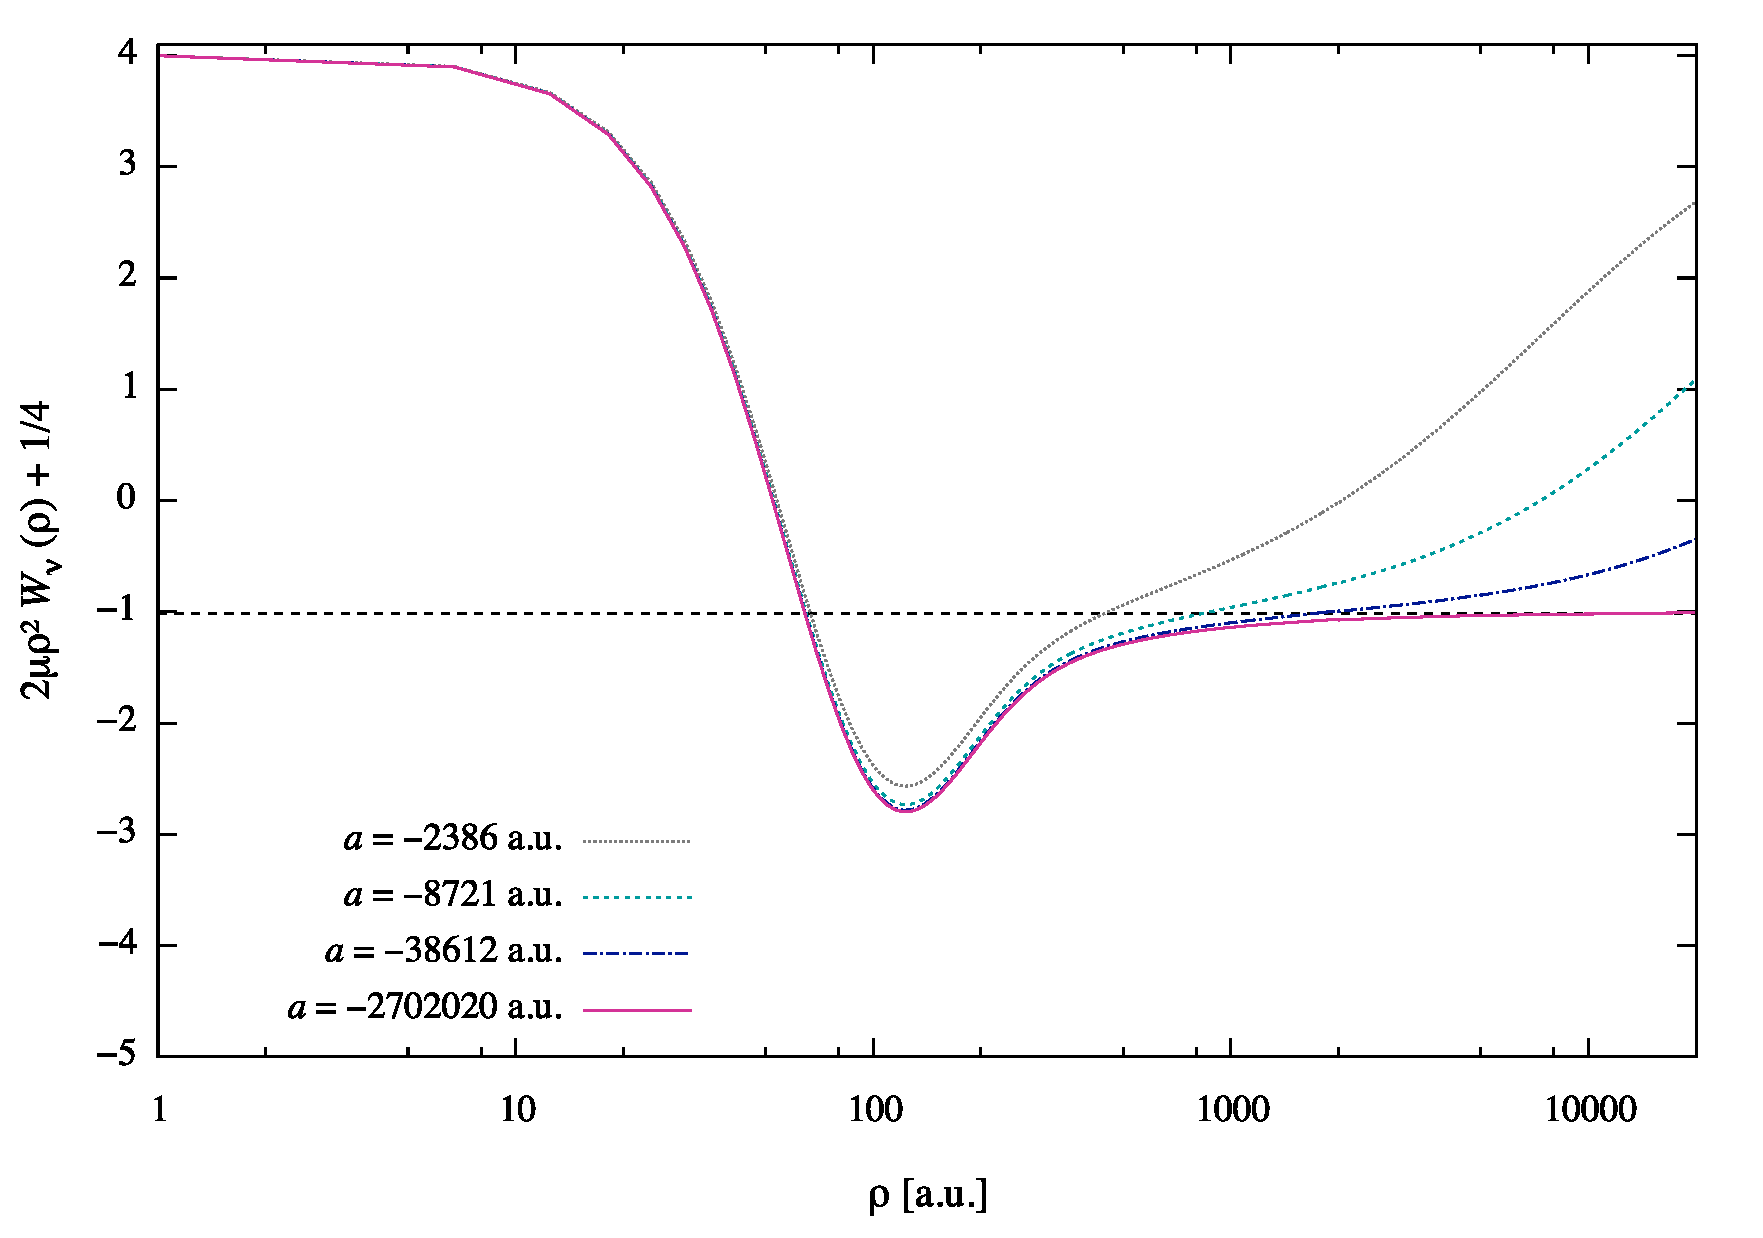
\includegraphics[width=\linewidth]{finite_negative_a.pdf}
	\caption{Three-body effective potentials for $a<0$. The horizontal dashed line is the universal value $-s_0^2$.}
	\label{fig:res_3}
\end{figure}

To further investigate the validity of the code we now compare our numerically calculated three-body effective potentials $\xi(\rho)$ for a number of finite $a$ states with the lowest energy eigenvalues $\nu_n(\rho)$ of the adiabatic hyperangular Faddeev equation for $a>0$ and $a<0$. These eigenvalues can be derived analytically in the limit of large $\abs{a}$ over the full hyperradial range and are determined by solving the transcendental equation \eqref{eq:transcendental}. The adiabatic eigenvalues $\nu_n(\rho)$ of \Cref{eq:faddeev_hyperang} are related to the three-body effective potentials calculated in this work through \Cref{eq:faddeev_effectivepot}. 

In \Cref{fig:faddeev} we present the lowest eigenvalues $\nu_0(\rho/\abs{a})$ calculated from \Cref{eq:transcendental} for $a>0$ and $a<0$. For both positive and negative $a$, the adiabatic states converge to the universal value $\nu_0(0) = -s_0^2$ in the region where $\rho/\abs{a}$ is small. For large $\rho/\abs{a}$, however, we observe that $\nu_0(\rho/\abs{a})$ for $a>0$ takes on a parabolic asymptotic form, which corresponds to a state with one diatomic molecule and one free atom, whereas for $a<0$ the state can be seen to approach $\nu_0=4$, thus corresponding to the lowest kinetic energy eigenvalue for three free atoms.  

\begin{figure}[htbp!]
	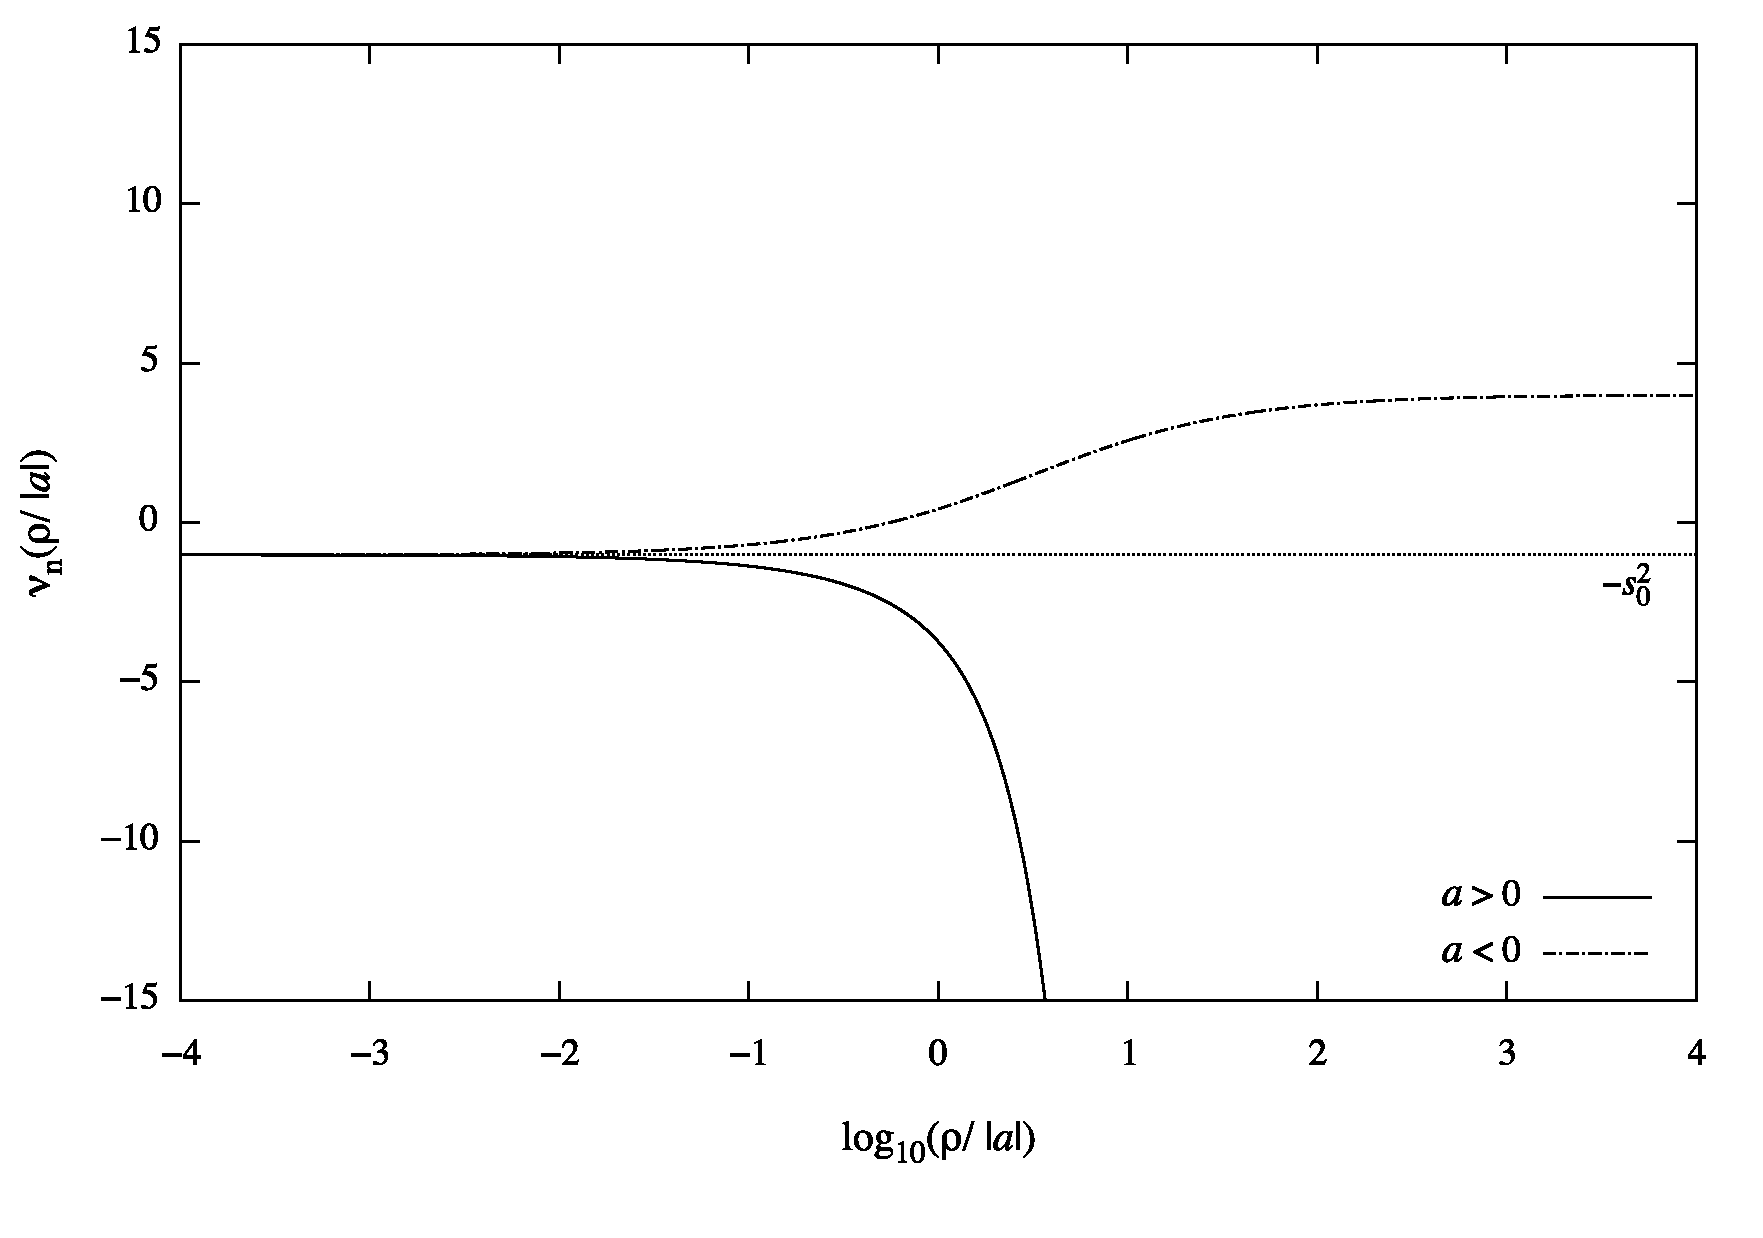
\includegraphics[width=\linewidth]{faddeev.pdf}
	\caption{Eigenvalues $\nu_0(\rho/\abs{a})$ of the hyperangular Faddeev equation \eqref{eq:faddeev_hyperang}, for $a>0$ (the solid line) and $a<0$ (the dash-dotted line).}
	\label{fig:faddeev}
\end{figure}

In \Cref{fig:conv} we show the numerical three-body effective potentials $\xi(\rho)$ plotted as functions of $\rho/\abs{a}$ for four different $a$ in comparison with the analytical eigenvalues $\nu_0(\rho/\abs{a})$. The calculations were performed using an increasingly refined mesh and a hyperradial grid with $250$ points. Each potential was obtained using an equal number of B-splines in each hyperangular coordinate ($N_{\theta} = N_{\phi}$). The effective potentials in the upper two panels are shown for \subref{fig:conv_a} $a=-2385$ a.u. and \subref{fig:conv_b} $a=-8720$ a.u., together with the analytically derived eigenvalues $\nu_0(\rho/\abs{a})$ of \Cref{eq:faddeev_hyperang} for $a<0$ (the dashed black lines in the upper panels). The hyperradial range, for which the numerical potentials converge to the analytical potential, can be seen to increase as a function of mesh resolution. For the state where the magnitude of $a$ is smaller, we observe that the hyperradial range, over which the numerical potentials converge towards the analytical values, is larger. For the potentials calculated using the mesh with a total of $40^2$ B-splines, convergence out to $\rho/\abs{a} \approx 40$ and $8$ can be seen in \subref{fig:conv_a} and \subref{fig:conv_b}, respectively.  

The calculations for positive $a$ are shown in the lower two panels in \Cref{fig:conv}, together with the analytically derived eigenvalues $\nu_0(\rho/\abs{a})$ for $a>0$ (the solid black lines in the lower panels). Panel \subref{fig:conv_c} contains the three-body effective potentials $\xi(\rho)$ for $a=1018$ a.u. Here we observe that the convergent behaviour of $\xi(\rho)$ deviates from the effective potential $\nu_0(\rho/\abs{a})$. The slightly different form in the parabolic divergency of the curves is due to a discrepancy between the exact two-body energy $E_{2b}$, which is given in \Cref{eq:exact_2b}, and the energy of the universal shallow dimer $-E_D=-1/ma^2$. To illustrate this more clearly we have in \Cref{fig:twobody} written the adiabatic potentials $\nu_{n}(\rho)$ on the form  

\begin{equation}
\widetilde{W}_n(\rho) =\frac{\nu_n(\rho)-1/4}{2\mu \rho^2},
\end{equation}
and plotted the three-body effective Faddeev potential $\widetilde{W}_{0}(\rho)$, together with the numerically calculated three-body effective potentials $W_{0}(\rho)$, as functions of $\rho/a$. The numerical potentials can be seen to converge to the exact energy of the binary subsystem (a dashed black line marked $E_{2b}$ in the figure), while the Faddeev potential approaches the approximate energy of the universal dimer (a dashed black line marked $-E_D$ in the figure). Since the binding energy of the universal dimer is exact in the resonant limit $a \rightarrow \infty$, we expect that the discrepancy between the analytic and the numerical curves is reduced if $a$ is increased. In panel \subref{fig:conv_d} in \Cref{fig:conv} we show that the potential curves for $a=5655$ a.u. are converging, as the number of B-splines is increased, to a parabolically divergent curve more similar to $\nu_0(\rho/\abs{a})$. The corresponding effective potentials $W_{0}(\rho)$ and $\widetilde{W}_0(\rho)$ are shown as functions of $\rho/a$ in \Cref{fig:twobody_5}, where we observe that the gap between the two curves in the asymptotic region is significantly smaller than the gap shown in \Cref{fig:twobody}. 

By comparing the left and right panels in \Cref{fig:conv} it appears that the hyperradial range for convergence generally is larger for the states with smaller $\abs{a}$. We suspect that this discrepancy is due to the knot point placement, but this has not been verified yet. 

\begin{figure}[htbp!]
	\centering{\phantomsubcaption\label{fig:conv_a}\phantomsubcaption\label{fig:conv_b}\phantomsubcaption\label{fig:conv_c}\phantomsubcaption\label{fig:conv_d}}
	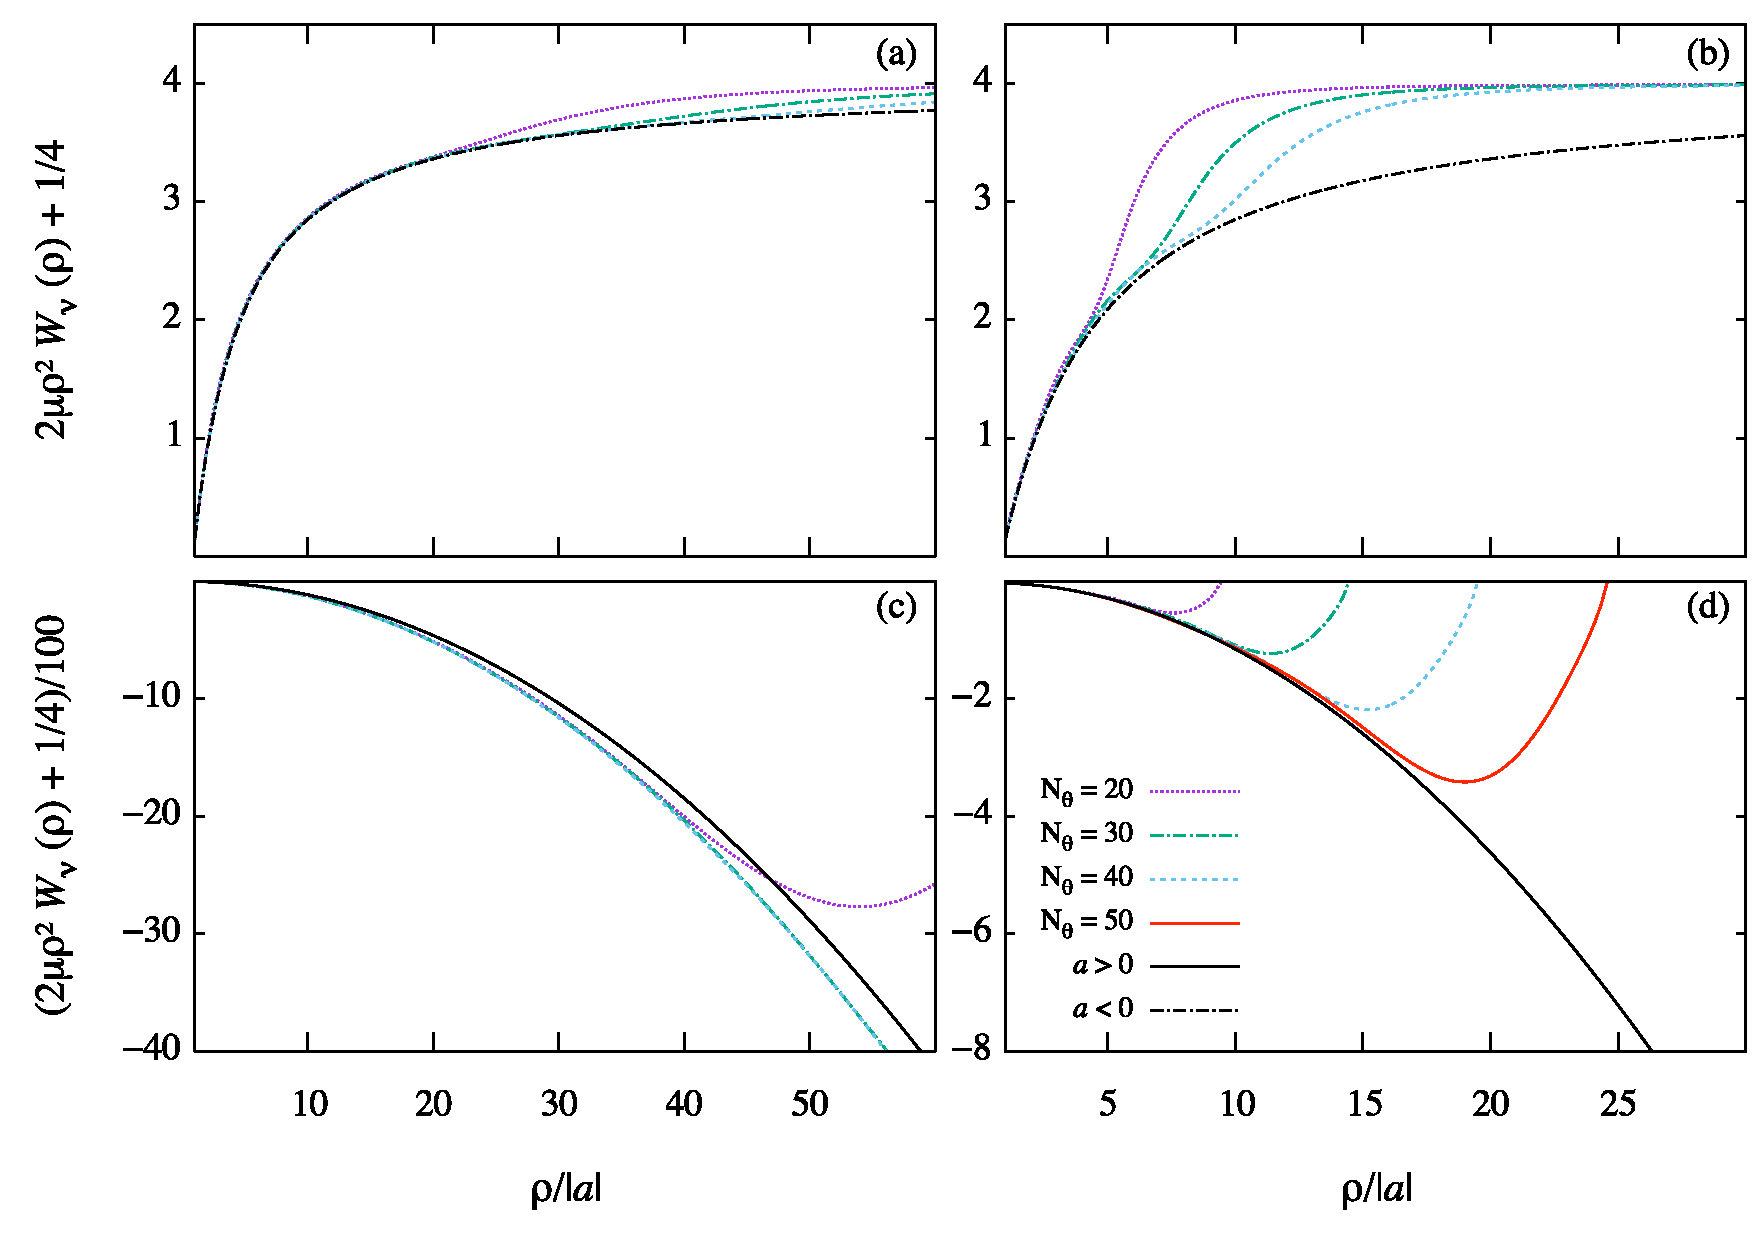
\includegraphics[width=\linewidth]{conv2815.pdf}
	\caption{Three-body effective potentials $\xi(\rho)$, calculated using an increasing number of B-splines, are plotted as functions of $\rho/\abs{a}$. In the upper two panels we show the potentials for \subref{fig:conv_a} $a=-2385$ a.u. and \subref{fig:conv_b} $a=-8720$ a.u., together with the analytic eigenvalues $\nu_0(\rho/\abs{a})$ of \Cref{eq:faddeev_hyperang} for $a<0$ (the black dash-dotted lines). In the lower two panels we show the potentials for \subref{fig:conv_c} $a=1018$ a.u. and \subref{fig:conv_d} $a=5655$ a.u. together with $\nu_0(\rho/\abs{a})$ for $a>0$ (the black solid lines). The numerically calculated potentials shown in panel \subref{fig:conv_d} appear to approximately converge to $\nu_0(\rho/\abs{a})$, while the potentials for $a=1018$ a.u. in panel \subref{fig:conv_c} can be seen to converge to a slightly different form than $\nu_0(\rho/\abs{a})$.}\label{fig:conv}
\end{figure}

\begin{figure}[htbp!]
	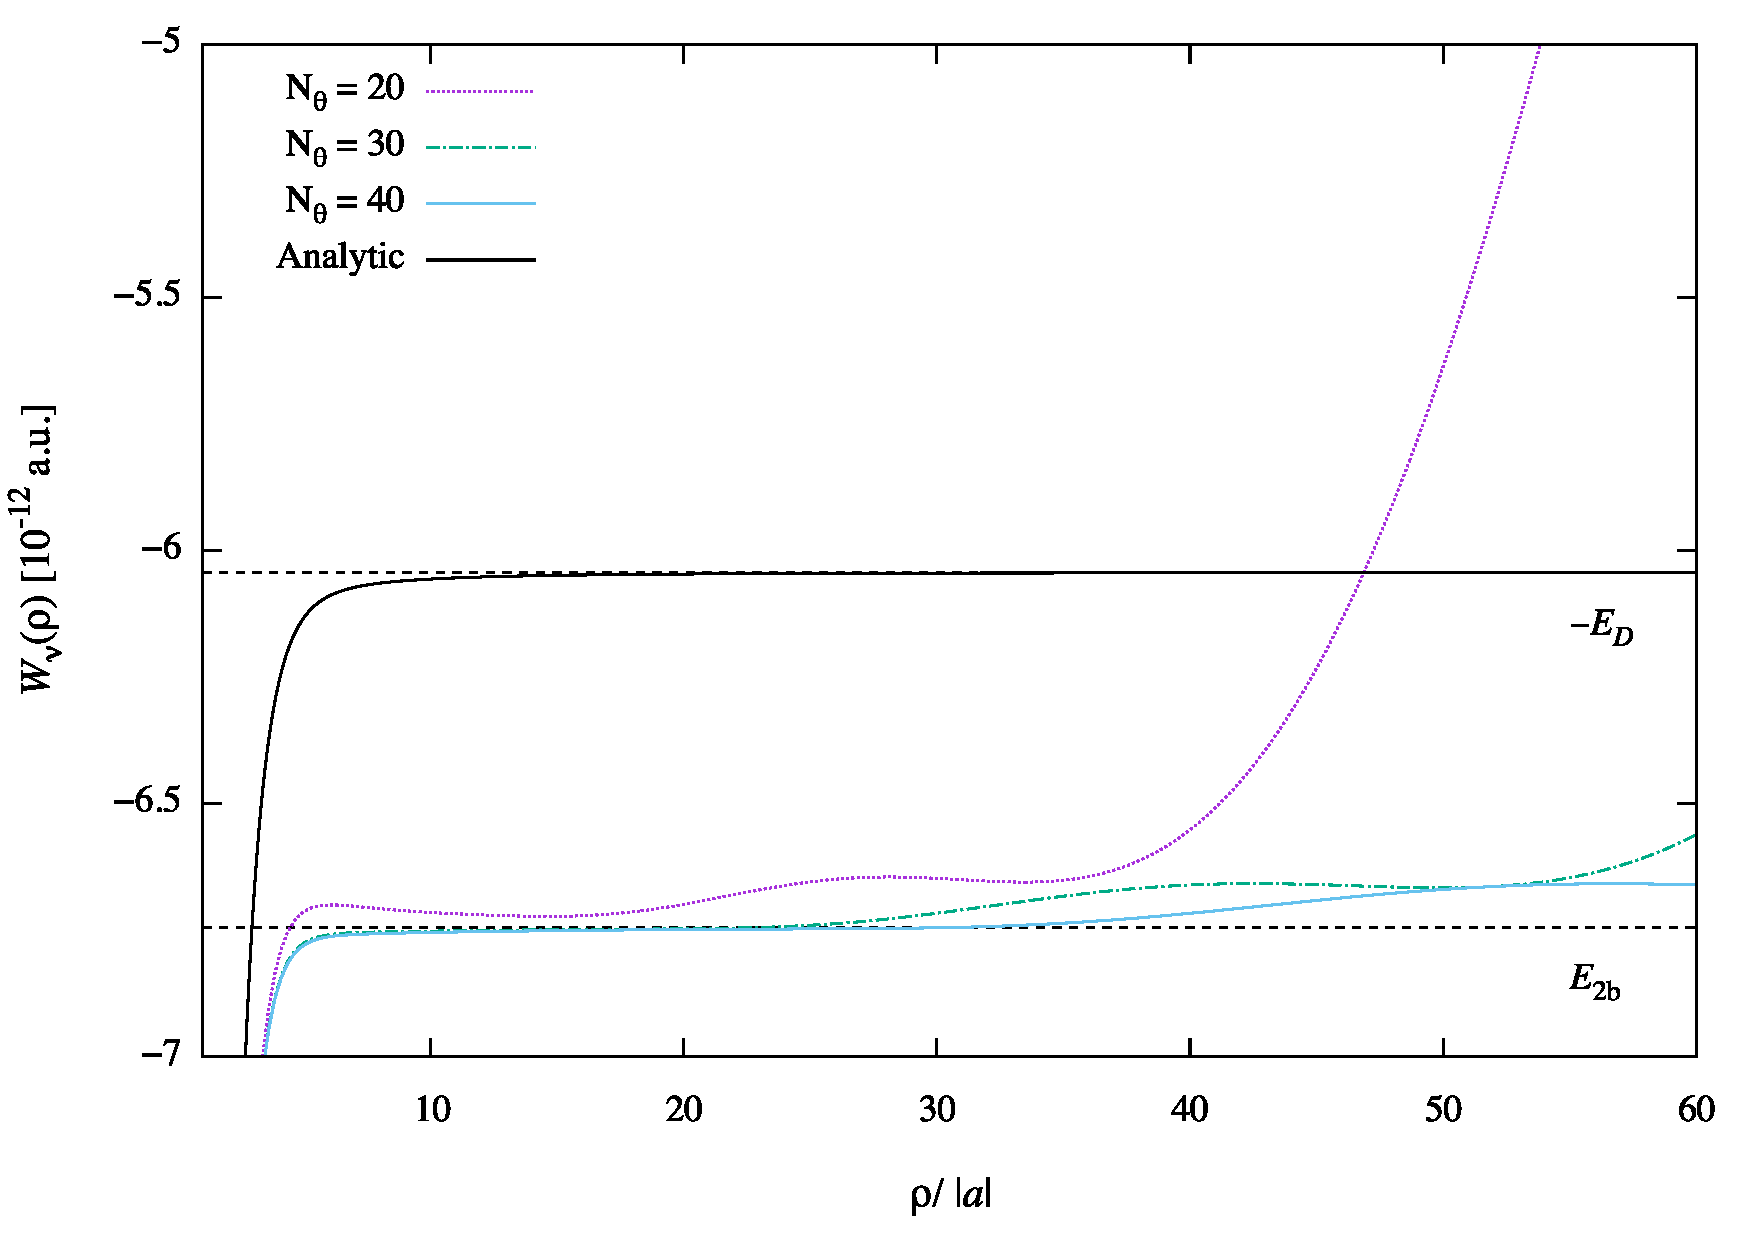
\includegraphics[width=\linewidth]{twobodyenergy.pdf}
	\caption{Three-body effective potentials $W_0(\rho)$ and $\widetilde{W}_0(\rho)$ for $a=1018$ a.u. are plotted as functions of $\rho/a$. The numerically calculated potentials $W_0(\rho)$ can be seen to converge asymptotically to the exact two-body bound energy $E_{2b}$, while the analytically derived potential $\widetilde{W}_0(\rho)$ approaches the approximate energy of the universal dimer $-E_D$.}
	\label{fig:twobody}
\end{figure} 

\begin{figure}[!ht]
	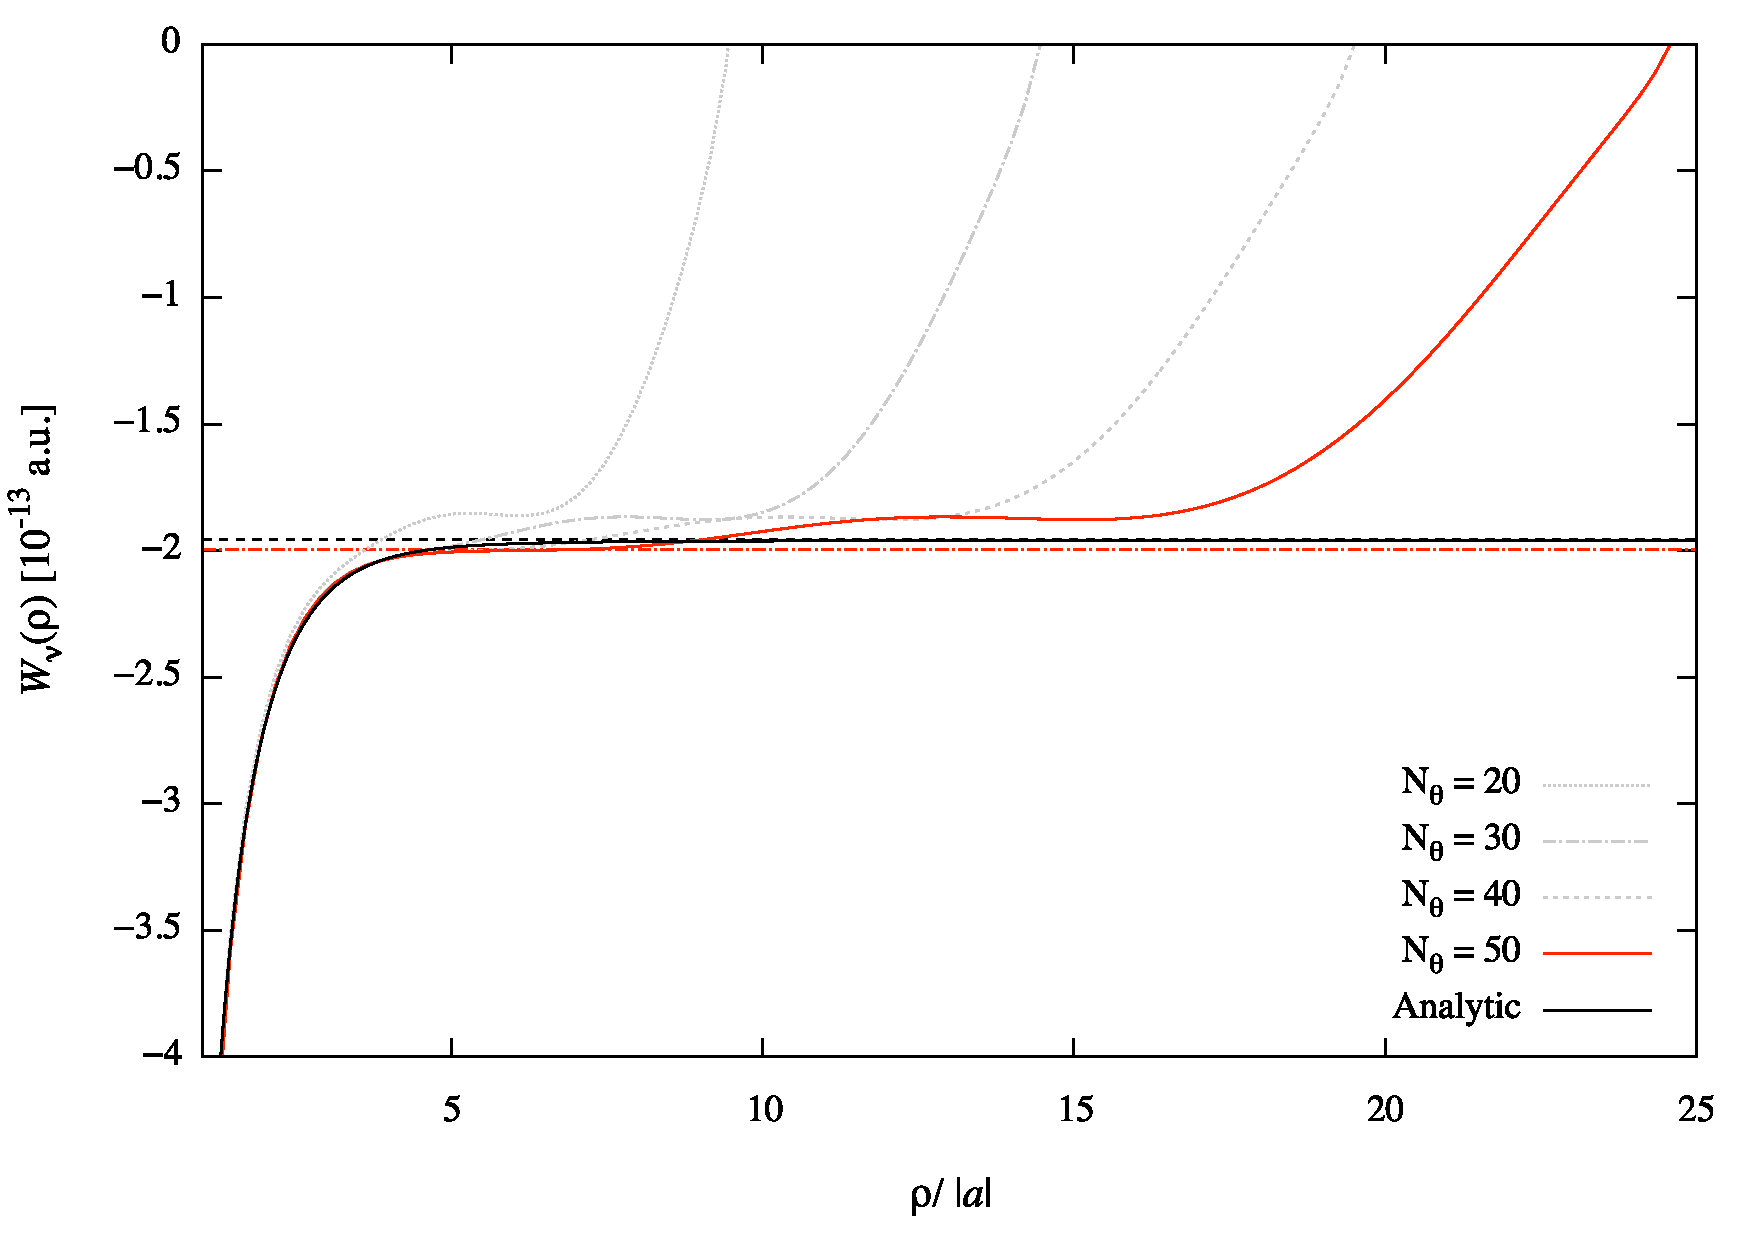
\includegraphics[width=\linewidth]{twobodyenergy_5.pdf}
	\caption{Three-body effective potentials $W_0(\rho)$ and $\widetilde{W}_0(\rho)$ for $a=5655$ a.u. are plotted as functions of $\rho/a$. The numerical potential $W_0(\rho)$ calculated with $N_{\theta} = 50$ is highlighted in red and can be seen to converge asymptotically to the exact two-body bound energy $E_{2b}$ (the dash-dotted red line), while the effective potential $\widetilde{W}_0(\rho)$ approaches the approximate energy of the universal dimer $-E_D$ (the dashed black line).}
	\label{fig:twobody_5}
\end{figure}

In the following we will look closer into the structure of the Efimov-like effective potentials $W_{\nu}(\rho)$ for cases where $a$ is finite and when $a \rightarrow \pm \infty$. From \Cref{eq:number_of_states} it is possible to predict the number of Efimov trimers that can be formed for each potential setting. With the current interaction range the magnitude of the scattering length needs to be larger than $\sim 1250$ a.u. to anticipate at least one Efimov state. For illustrative purposes, however, we show two cases where $\abs{a} \sim 200$ a.u., since these exemples in a clear way show the Efimov-like features of the potentials.     

The adiabatic potential curves shown in \Cref{fig:Wpos} were numerically calculated with a potential strong enough to support a single $s$-wave bound state and the potential depth $d$ was tuned to yield a scattering length of $a=252$ a.u. The adiabatic potential curves $W_{\nu}(\rho)$ with $\nu = 0-4$ are plotted as functions of the hyperradius $\rho/a$, where the Efimov channel is the lowest potential curve with channel index $\nu = 0$, which in the asymptotic region $\rho/a\gtrsim1$ converges to the two-body $s$-wave binding energy. All higher lying channels $\nu>1$ are repulsive everywhere and correspond to three-body continuum channels. As the potential depth parameter $d$ is moved towards pole $\mathrm{I}$ from the right and $a \rightarrow \infty$ the energy of the two-body bound state vanishes and the Efimov channel becomes a purley attractive $\rho^{-2}$ potential for $\rho>r_0$. 

Similarly, in \Cref{fig:Wneg} the adiabatic potential curves for $a<0$ with $\nu = 0-4$ is shown. The potential depth $d$ was in this case tuned to yield a scattering length of $a=-224$ a.u. The lowest potential curve with channel index $\nu = 0$, which asymptotically converges to the three-body continuum, corresponds to the Efimov channel. In this case, the three-body interaction has a potential barrier with a maximum located at $\rho/\abs{a} \approx 2$, while in the intermediate range $r_0 \lesssim \rho \lesssim a$ the potential is attractive. A magnification of the barrier region is shown in the inset in \Cref{fig:Wneg}. 

\begin{figure}
	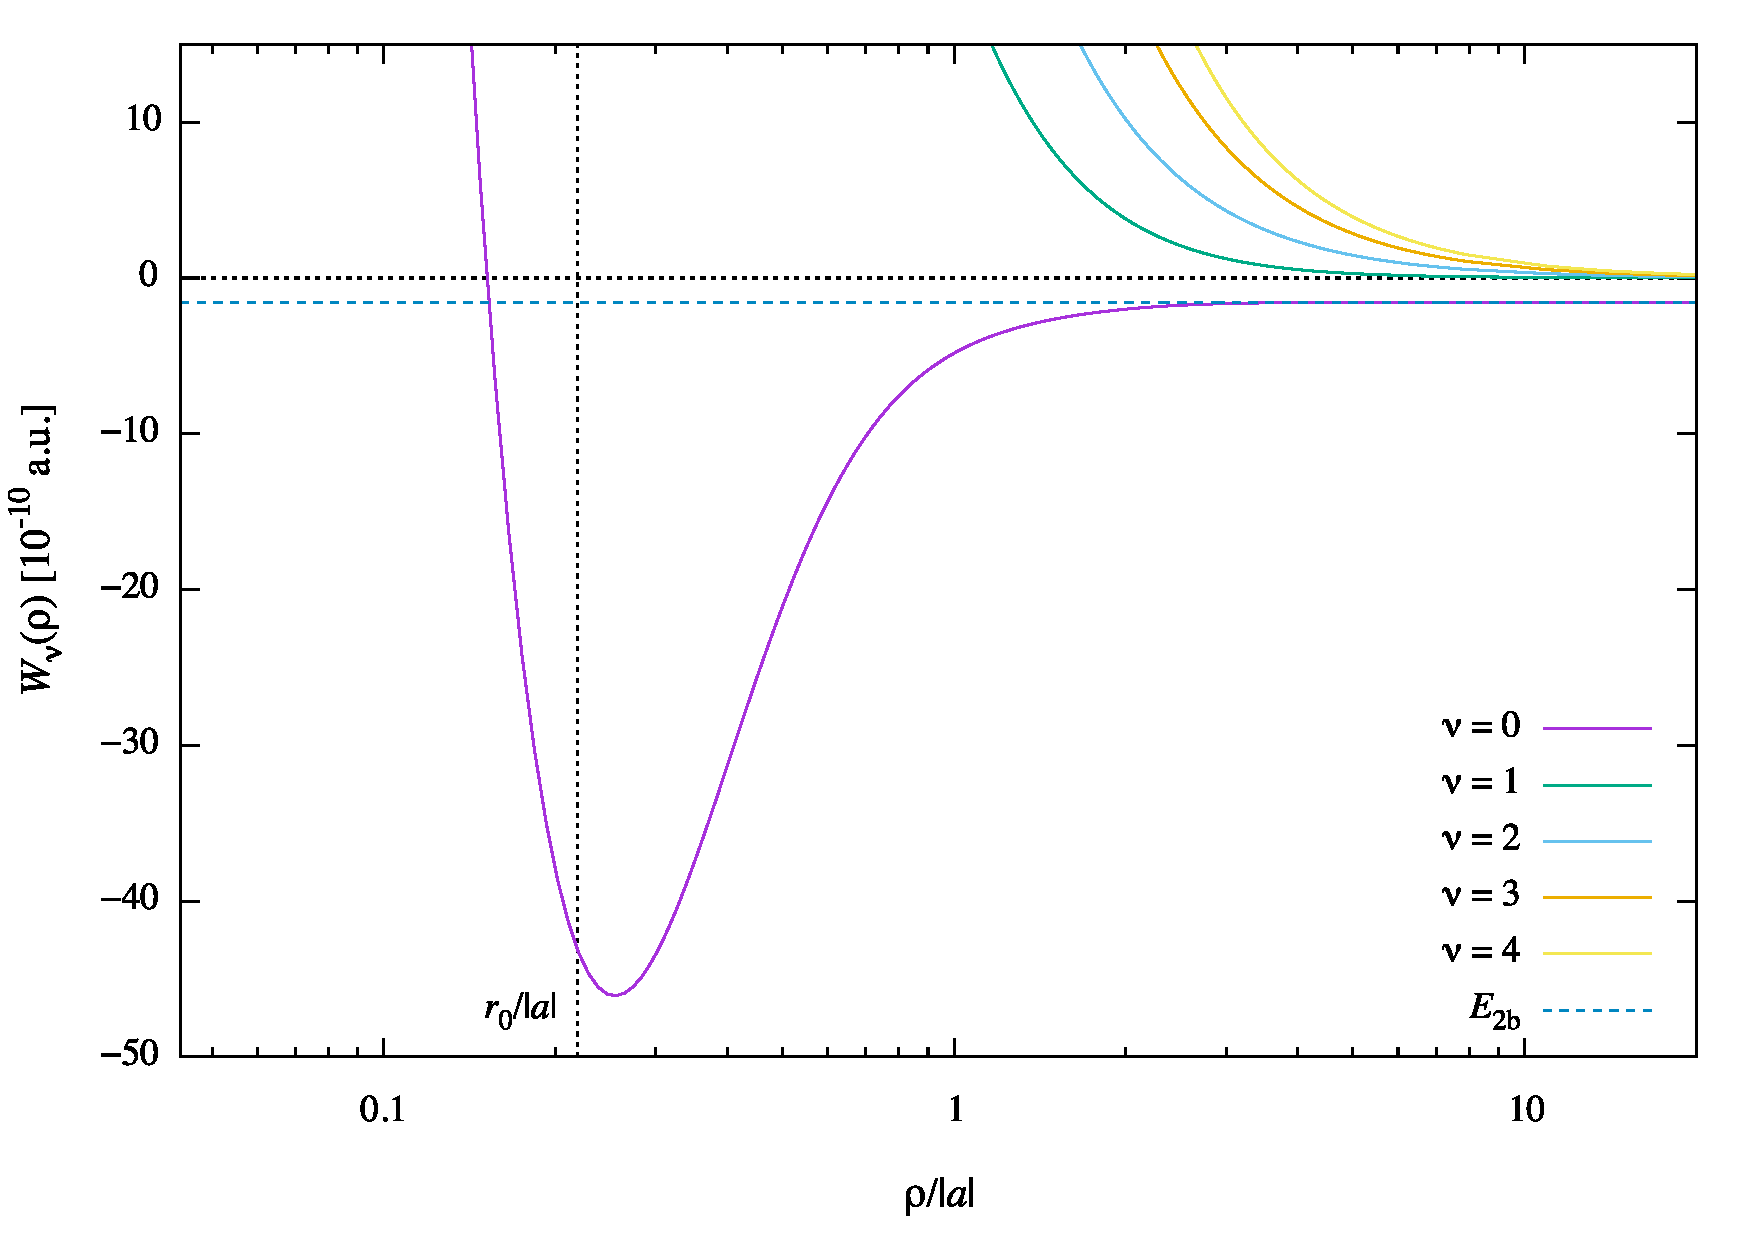
\includegraphics[width=\linewidth]{Wpos2.pdf}
	\caption{Three-body effective potentials for $a=252$ a.u. The horizontal blue dashed line is the energy of the dimer.}
	\label{fig:Wpos}
\end{figure}

\begin{figure}
	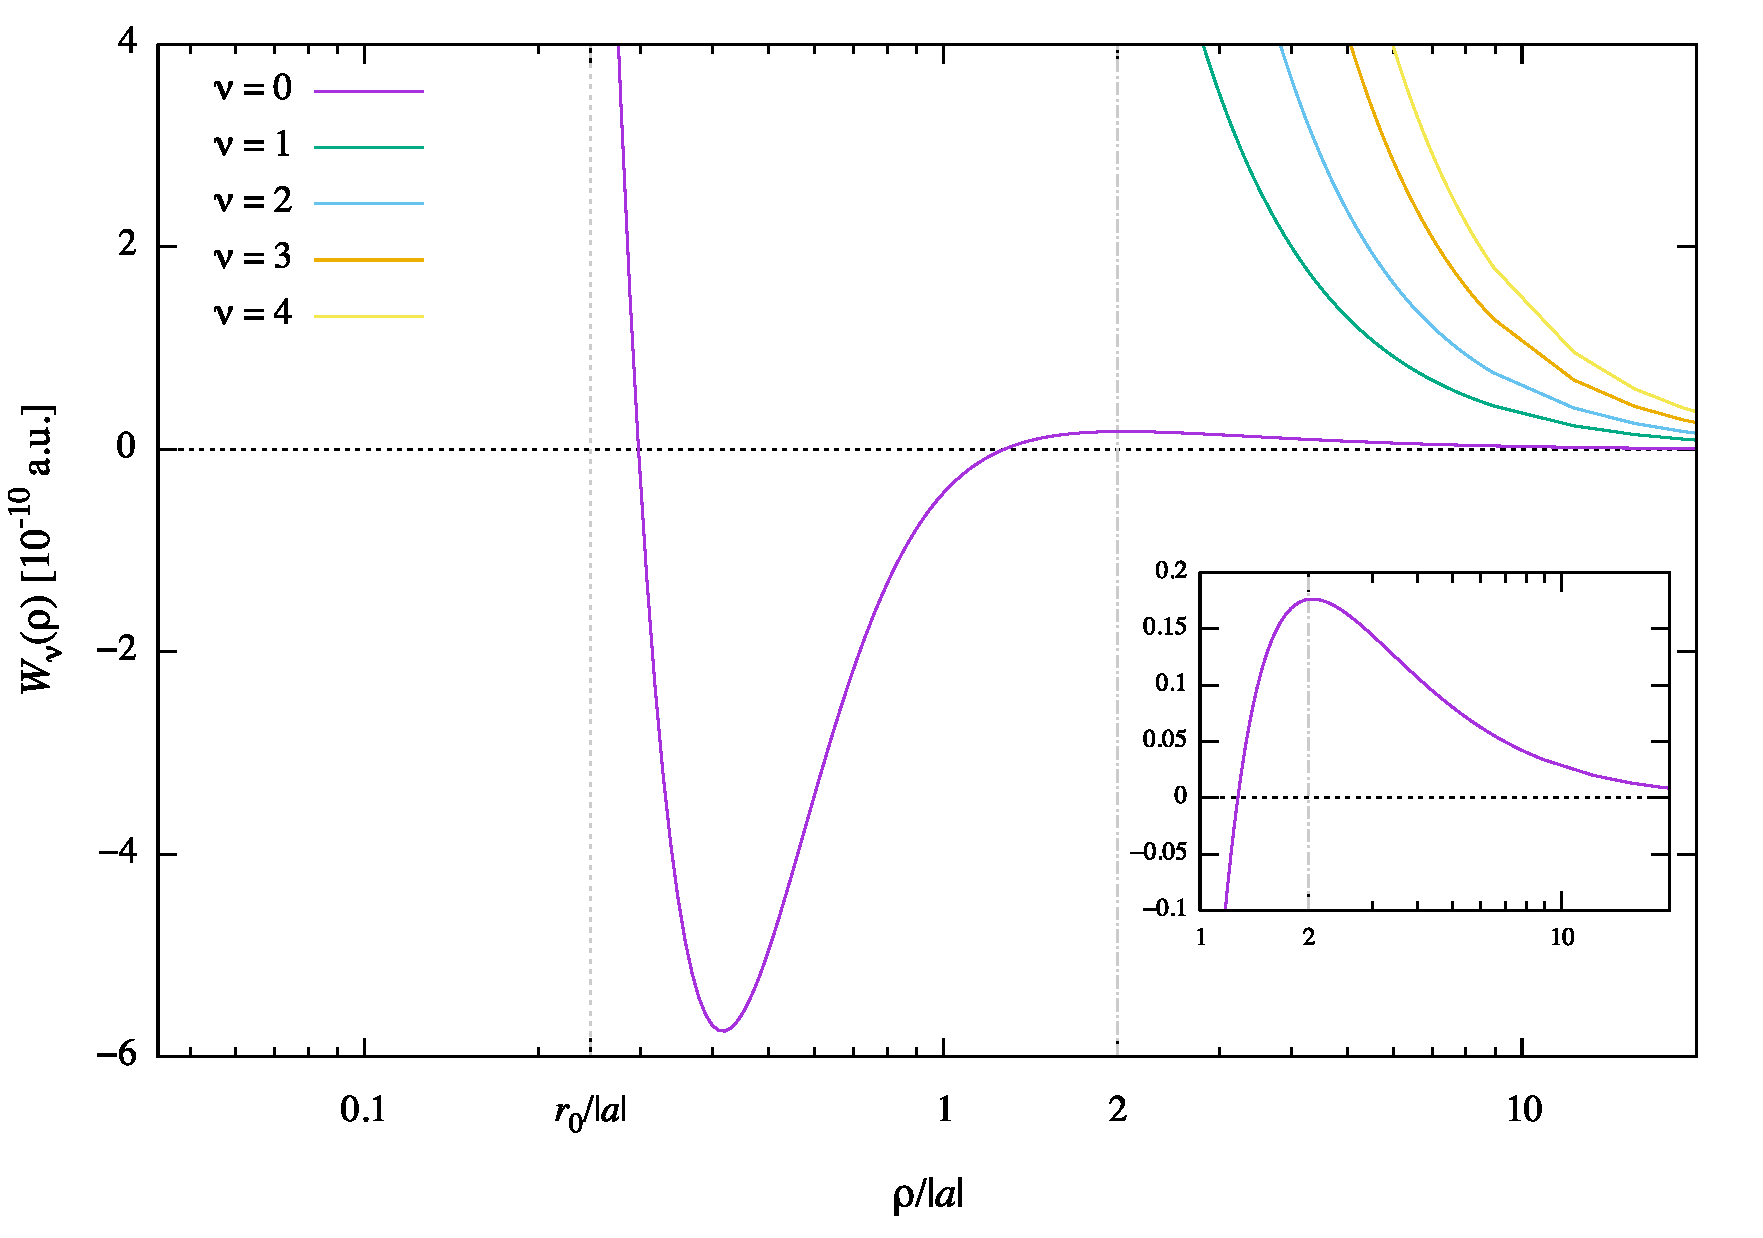
\includegraphics[width=\linewidth]{Wneg2.pdf}
	\caption{Three-body effective potentials for $a=-224$ a.u. The potential $\nu = 0$ has a potential barrier with a maximum located at $\rho/\abs{a} \approx 2$ (shown magnified in the inset).}
	\label{fig:Wneg}
\end{figure}

In \Cref{fig:barrier} we show the effective potentials calculated with increasing values of $d$ starting from the left-hand side ($a<0$) and ending on the right-hand side ($a>0$) of pole $\mathrm{I}$. The potentials calculated for $a<0$ are here shown in blue, while the ones calculated for $a>0$ are shown in red. 

A common feature for all Efimov-like effective potentials with negative scattering lengths is the kind of centrifugal barrier, with a long-range maximum, which we observed earlier in \Cref{fig:Wneg}. For the three-body wave function incident from $\rho \rightarrow \infty$ to get to the region $\rho<\abs{a}$, it must tunnel through this barrier. The presence of a centrifugal barrier indicates that it is possible to have a trimer shape resonance at $E>0$ for certain negative values of $a$. A shape resonance is a long-lived metastable state in which the three-body system is trapped in the region $\rho<\abs{a}$ due to the shape of the potential barrier. If the three-body wave tunnels through the barrier and the formed metastable state allows for the three atoms to be close to each other for an extended period of time before they fly apart, there is an increased probability that the system will relax into a deeply bound dimer and a free atom, with the free atom carrying away the excess kinetic energy. When the energy of the incident trimer matches a resonance, there is an enhanced barrier penetrability to form an Efimov resonance, which will cause an increased probability of the formation of deeply bound dimer states and high energy free atoms. Thus, in collision experiments with a trapped gas of ultracold atoms with tunable interactions, this recombination mechanism can cause resonantly enhanced atom losses at certain values of $a$ due to a sudden increase in the formation of atom-dimer states, because the energy conservation during the inelastic collision requires the binding energy released from the molecular formation to transform into kinetic energy of the relative motion between the dimer and the free atom, which subsequently causes them to escape the trap. This resonant enhancement of atom losses thus serves as a fingerprint of the elusive Efimov trimer states. 

When $d$ approaches the pole from the left and the value of $\abs{a}$ increases, the position of the barrier in the Efimov channel moves to larger $\rho$, while the barrier height is reduced. This is illustrated in the upper and lower inset in \Cref{fig:barrier}, where we show that as the scattering length is changed, the position of the barrier maxima grows proportional to $\abs{a}$ and moves to infinity when $a \rightarrow -\infty$, while the barrier height shrinks proportional to $1/a^2$ and vanishes at infinity. This means that as $\abs{a}$ increases the resonance energy decreases and at some particular $a$ it will coincide with the collision energy. When this occurs the recombination rate is strongly enhanced because the amplitude of the scattering wave function behind the barrier, where the Efimov channel couples to the atom-dimer channel, grows significantly larger on resonance \cite{Esry_2007}.

The ideal Efimov effect occurs when the barrier is at infinity and hence has zero height and none of the two-body subsystems are bound, or when a two-body subsystem of three particles supports a dimer at zero energy. This scenario is realized for states calculated with values of $d$ very close to the pole. 

In \Cref{fig:barrier} we show that our numerically calculated potentials for $a \rightarrow \pm \infty$ (the potentials labelled $a_3$ and $a_4$ in the figure) are essentially the same, with an attractive $1/\rho^2$ character. After crossing the pole, a further increase in $d$ will result in the typical asymptotic convergence towards the energy of the $s$-wave state just below the zero energy threshold (the potential labelled $a_5$), which will be shifted to lower energies as $d$ grows (the potential labelled $a_6$).  

In \Cref{fig:barrier_analytic} we show that the repulsive barrier, characteristic for Efimov resonances, is present also in the analytically derived effective potentials $\widetilde{W}_0(\rho)$ for $a<0$. The numerical and analytical potential curves for $a_1=-224$ a.u. and $a_2=-2385$ a.u. are here plotted as functions of $\rho$. In the inset we show that the barriers for the $a_2$ potentials are almost identical, with a maximum at $\rho \approx 2a_2$. There is a greater discrepancy for the $a_1$ potentials, as can be expected, since the analytical results are exact in the unitary limit $\abs{a} \rightarrow \infty$.

\begin{figure}
	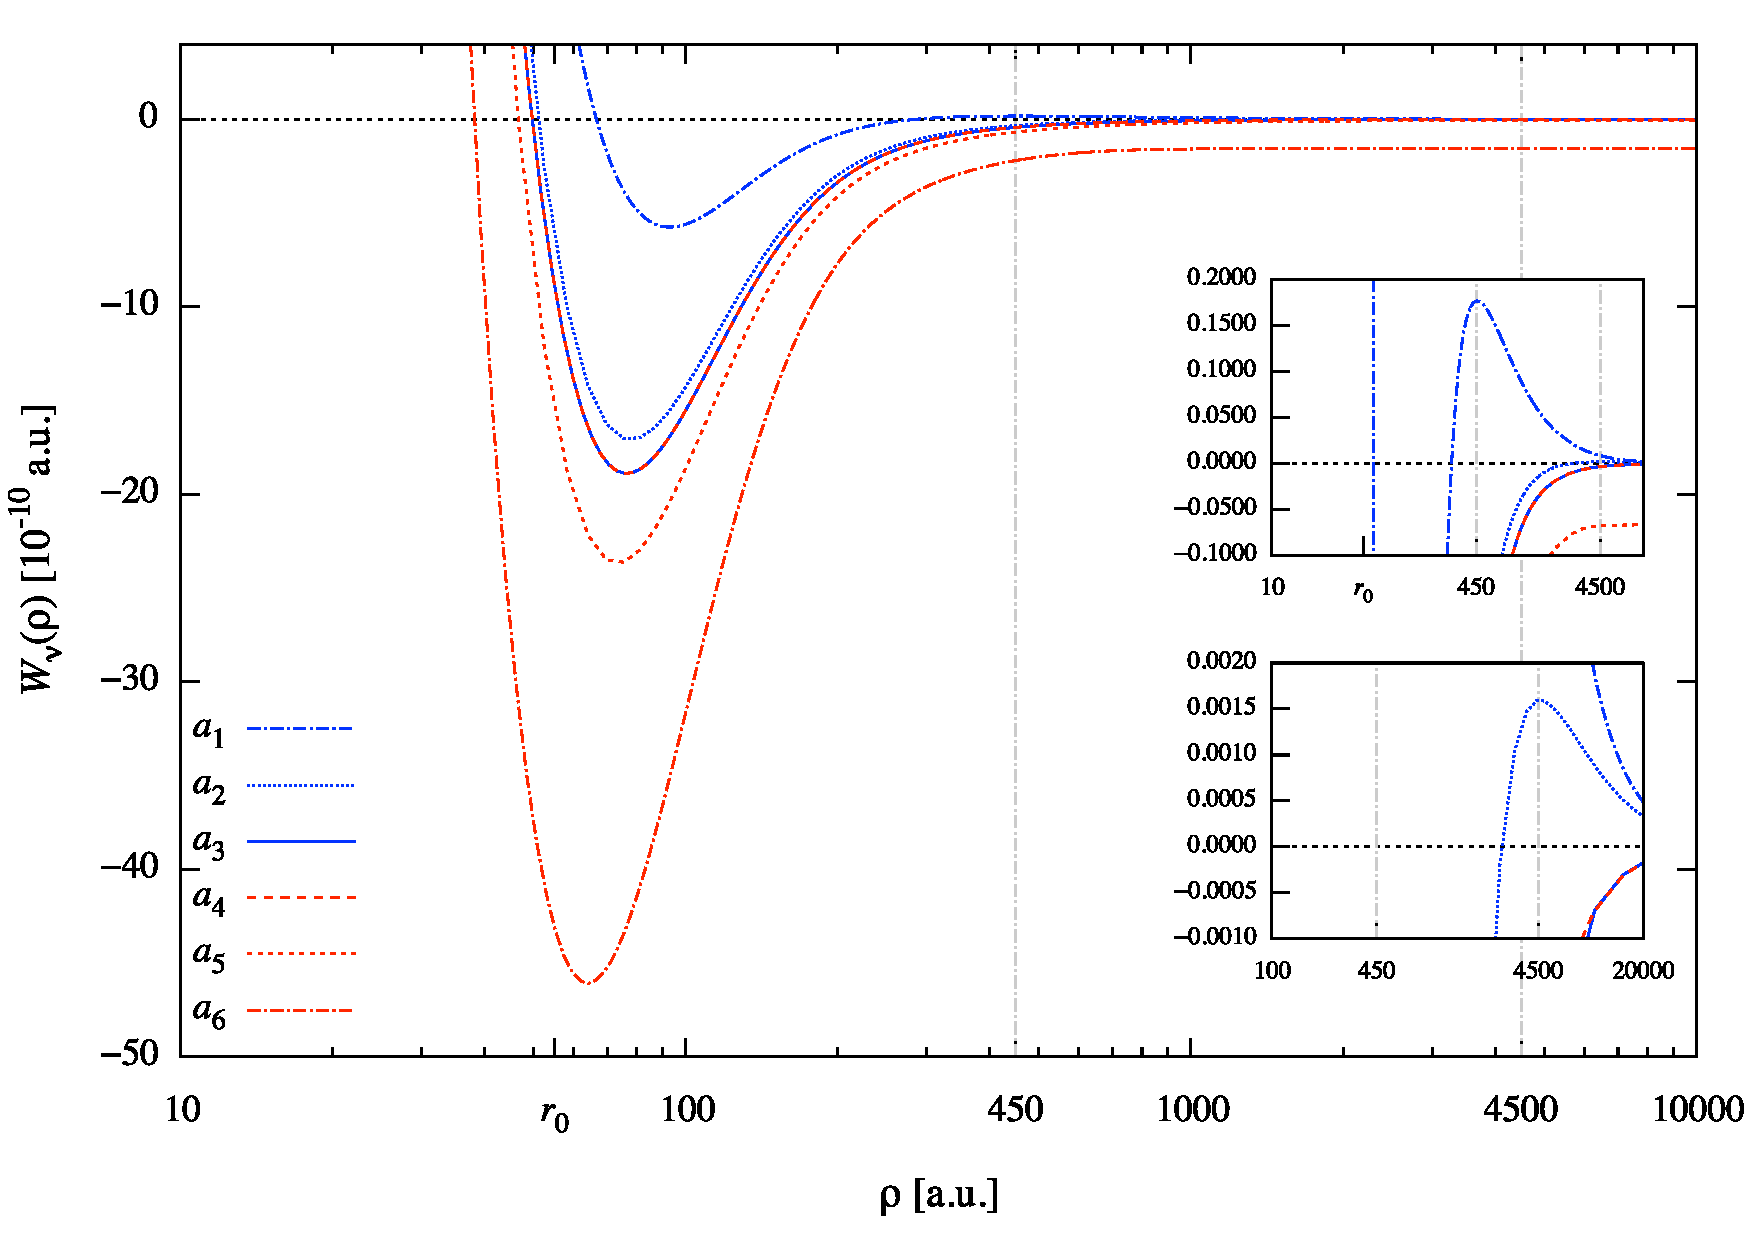
\includegraphics[width=\linewidth]{barrier.pdf}
	\caption{Three-body effective potentials calculated near pole $\mathrm{I}$. For $a<0$ the potentials are shown in blue, with $\abs{a_i}=224,2385,2702020$ a.u., where $i=1,2,3$. For $a>0$ the potentials are shown in red, with $a_i=1966590,1018,252$ a.u., where $i=4,5,6$. The upper inset shows the potential barrier for $a_1$ with a maximum located at $\rho \approx 450$ a.u. The lower inset shows the potential barrier for $a_2$ with a maximum located at $\rho \approx 4500$ a.u.}
	\label{fig:barrier}
\end{figure}

\begin{figure}
	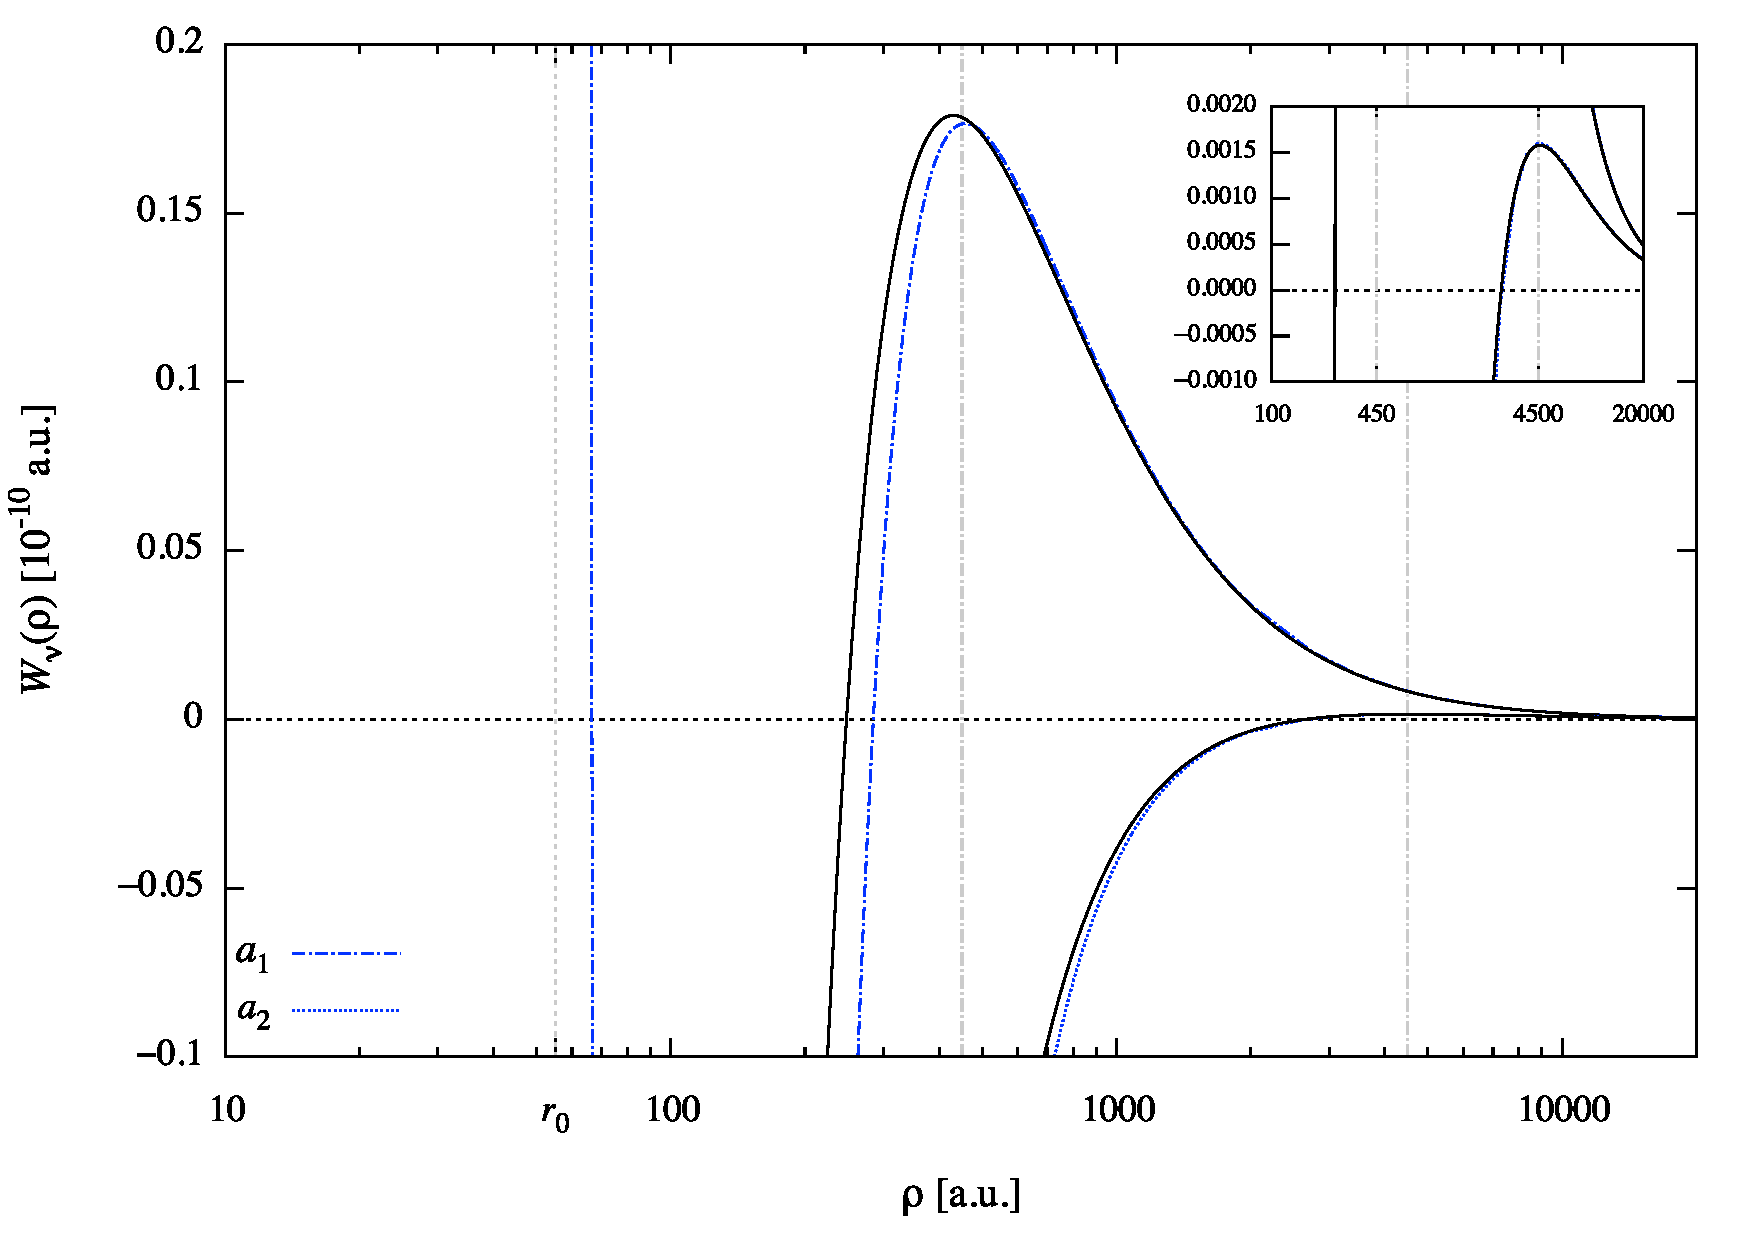
\includegraphics[width=\linewidth]{barrier_analytic.pdf}
	\caption{Three-body effective potentials $W_0(\rho)$ for $a_1=-224$ a.u. and $a_2=-2385$ a.u. are shown in blue together with the corresponding analytic potentials $\widetilde{W}_0(\rho)$, which are shown in black.}
	\label{fig:barrier_analytic}
\end{figure}